%!TEX root = ../NCVC.tex

\mysection{中級編}

\subsection{移動レイヤ}
\label{sec:move}
 NCVCには,原点レイヤ・切削レイヤの他にあと3つのレイヤ情報を読み込む機能があります.
ここではそのうちの2つ,加工開始位置指示レイヤと強制移動指示レイヤを解説します.

\subsubsection{加工開始位置指示レイヤ}
 図\ref{fig:sample3.pdf} のような加工を考えます.
原点はワーク矩形左下で円を内側から螺旋状に切削したいのですが,これだけでは思ったようなGコードを生成できません.

 NCVCは次の切削データを検索するとき,現在位置に最も近い座標を検索します.
したがって,原点から一番近い座標である外側の座標からGコードの生成を始めます.

 これを回避するため,NCVCでは[加工開始位置指示レイヤ]を用意しています.
CADでの作図で原点・切削の両レイヤとは別のレイヤを用意し,円を1つ作図して下さい.
レイヤ名も設定です.作図方法は原点指示と同じ,円の中心が加工開始座標となります.

 NCVCでの設定は【\ref{sec:ReadCAD} CADデータの読み込み】と同じです.
[読み込みレイヤ2]のタブをクリックし,NCVCが読み込むレイヤ名を設定して下さい(図\ref{fig:ReadSetup3.png}).
[読み込みレイヤ2]の設定は必須ではありませんが,CAD側で意図的に作図しない限りNCVCは読み込みませんので,常にこの設定にしても問題ありません.
レイヤ名は,原点・切削の両レイヤと同様に任意です.CAD側の設定と合わせて下さい.
加工開始指示を指示したシミュレーション結果を図\ref{fig:sample3.png} に示します.

\begin{minipage}{0.5\textwidth}
\begin{figure}[H]
\centering
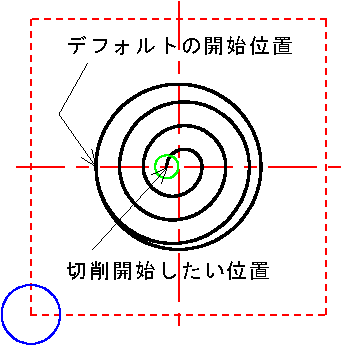
\includegraphics{No3/fig/start-crop.pdf}
\caption{サンプル図形}
\label{fig:sample3.pdf}
\end{figure}
\end{minipage}
\begin{minipage}{0.5\textwidth}
\begin{figure}[H]
\centering
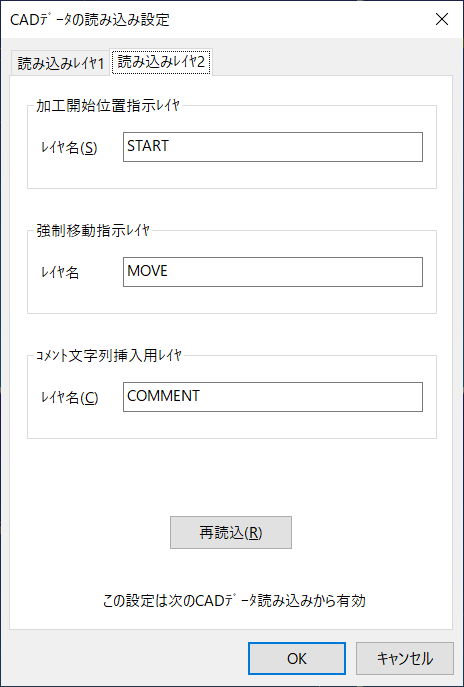
\includegraphics[scale=0.7]{No3/fig/ReadSetup3.png}
\caption{読み込みレイヤ設定}
\label{fig:ReadSetup3.png}
\end{figure}
\end{minipage}

\begin{figure}[H]
\centering
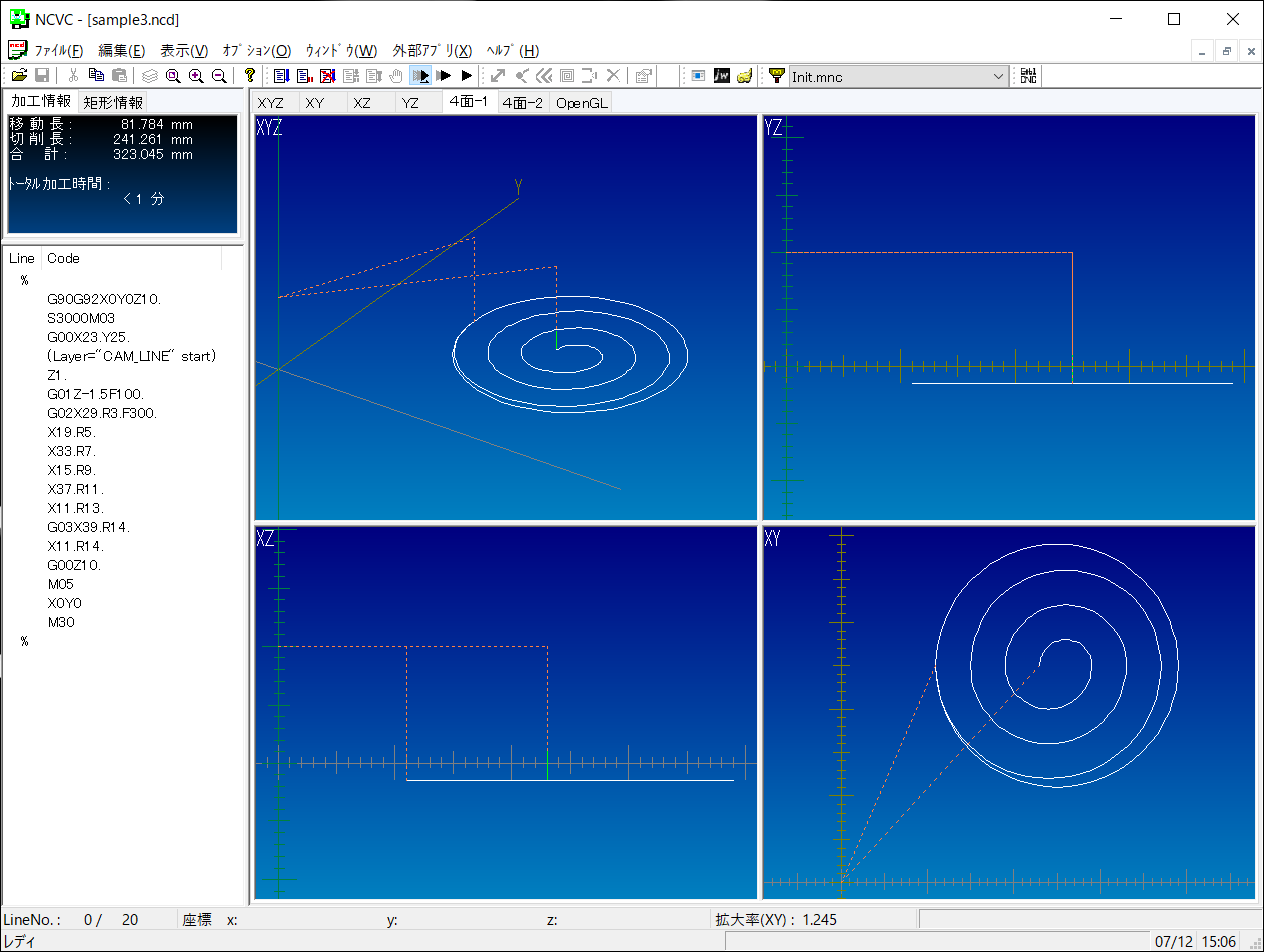
\includegraphics[scale=0.55]{No3/fig/sample3.png}
\caption{加工開始位置を追加したGコードシミュレーション画面}
\label{fig:sample3.png}
\end{figure}

 加工開始位置指示レイヤにはもう1つ機能があります.
例えば図\ref{fig:approach-img.png} のようなワーク形状の場合,原点からの最短移動ではワークに干渉してしまいます.
この場合,図\ref{fig:approach.pdf} のように干渉しないような移動軌跡を加工開始位置指示レイヤに作図することで,原点からの移動動作を制御することができます.
Z軸の初期座標を上げることで回避できる場合もあります.用途に応じてご使用下さい.

\begin{minipage}{0.5\textwidth}
\begin{figure}[H]
\centering
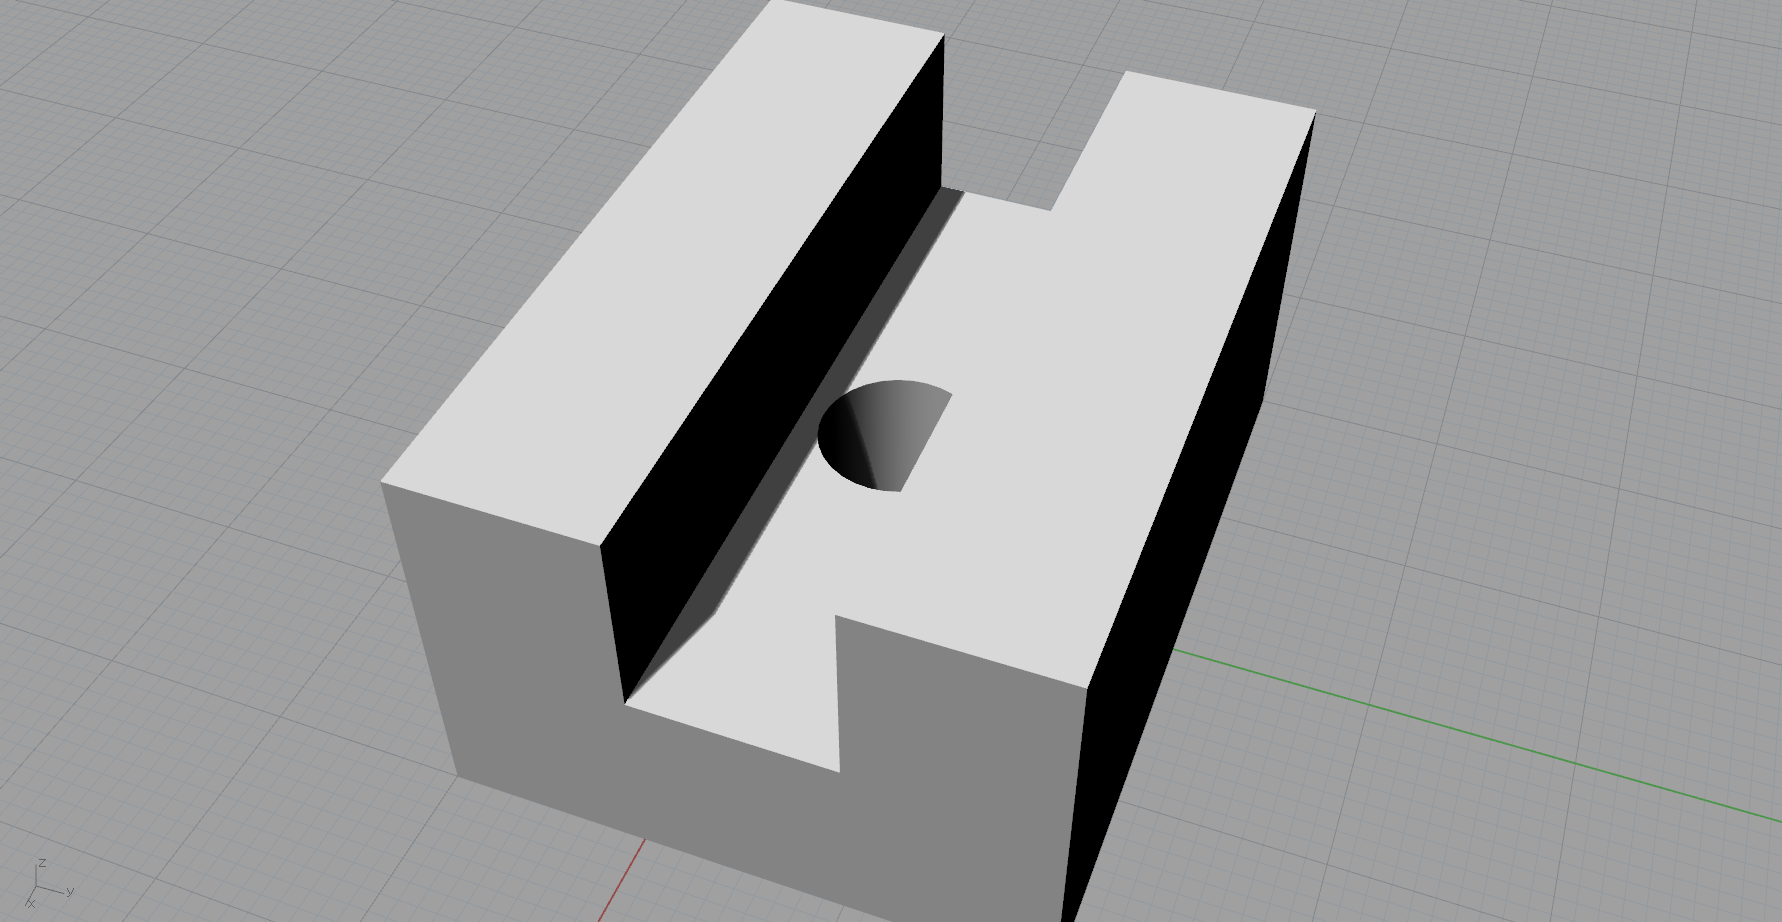
\includegraphics[width=\textwidth]{No3/fig/approach-img.png}
\caption{サンプルイメージ図}
\label{fig:approach-img.png}
\end{figure}
\end{minipage}
\begin{minipage}{0.5\textwidth}
\begin{figure}[H]
\centering
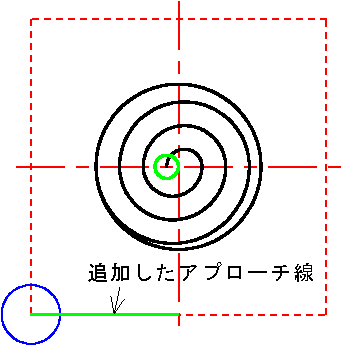
\includegraphics{No3/fig/approach-crop.pdf}
\caption{アプローチ線}
\label{fig:approach.pdf}
\end{figure}
\end{minipage}

\begin{figure}[H]
\centering
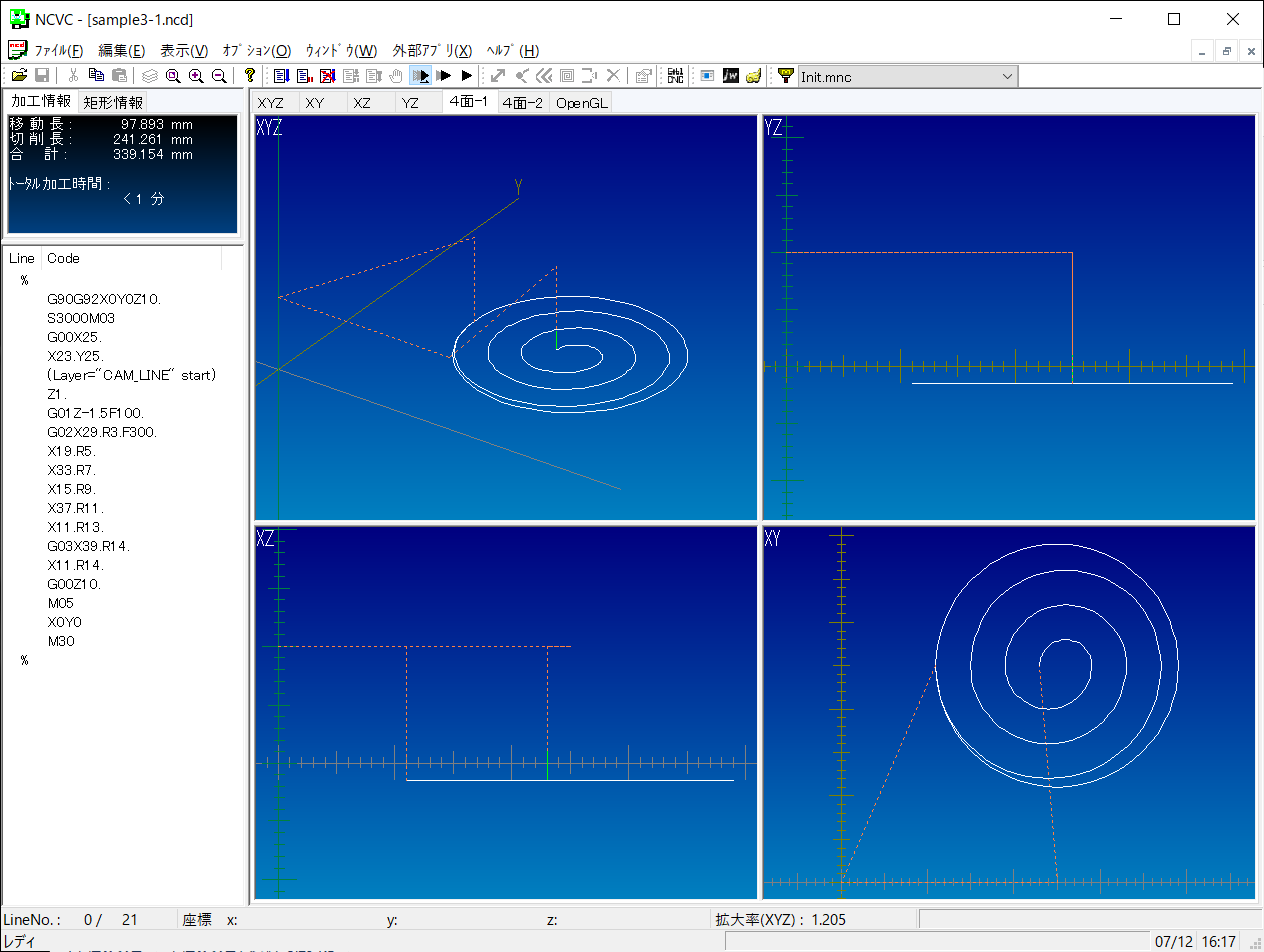
\includegraphics[scale=0.55]{No3/fig/sample3-1.png}
\caption{アプローチ線を追加したGコードシミュレーション画面}
\label{fig:sample3-1.png}
\end{figure}

\subsubsection{強制移動指示レイヤ}
 図\ref{fig:sample3-1.png} のシミュレーション結果を見ても解る通り,原点へ戻るときもワークと干渉してしまう可能性があります.
加工開始位置指示レイヤは,最初の加工位置やアプローチを指示するものでしたが,
強制移動指示レイヤは,次の切削データの検索途中でNCVCに移動を指示する情報となります.
つまり,次の切削領域への移動,Z軸の上下が必要なときに強制移動指示レイヤが参照されます.

\begin{minipage}[t]{0.5\textwidth}
 強制移動指示レイヤは線データのみを認識します.
図\ref{fig:ReadSetup3.png} で設定した移動レイヤに作図して下さい.
また,必ず切削データと接続されていなければなりません.
図\ref{fig:move.pdf} は切削が終わったあとの移動軌跡を作図したものです.
\end{minipage}
\begin{minipage}[t]{0.5\textwidth}
\vspace*{-2zh}
\begin{figure}[H]
\centering
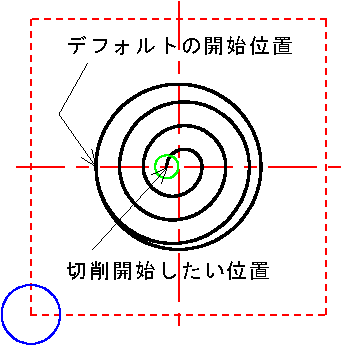
\includegraphics{No3/fig/move-crop.pdf}
\caption{強制移動指示レイヤを追加}
\label{fig:move.pdf}
\end{figure}
\end{minipage}

\begin{figure}[H]
\centering
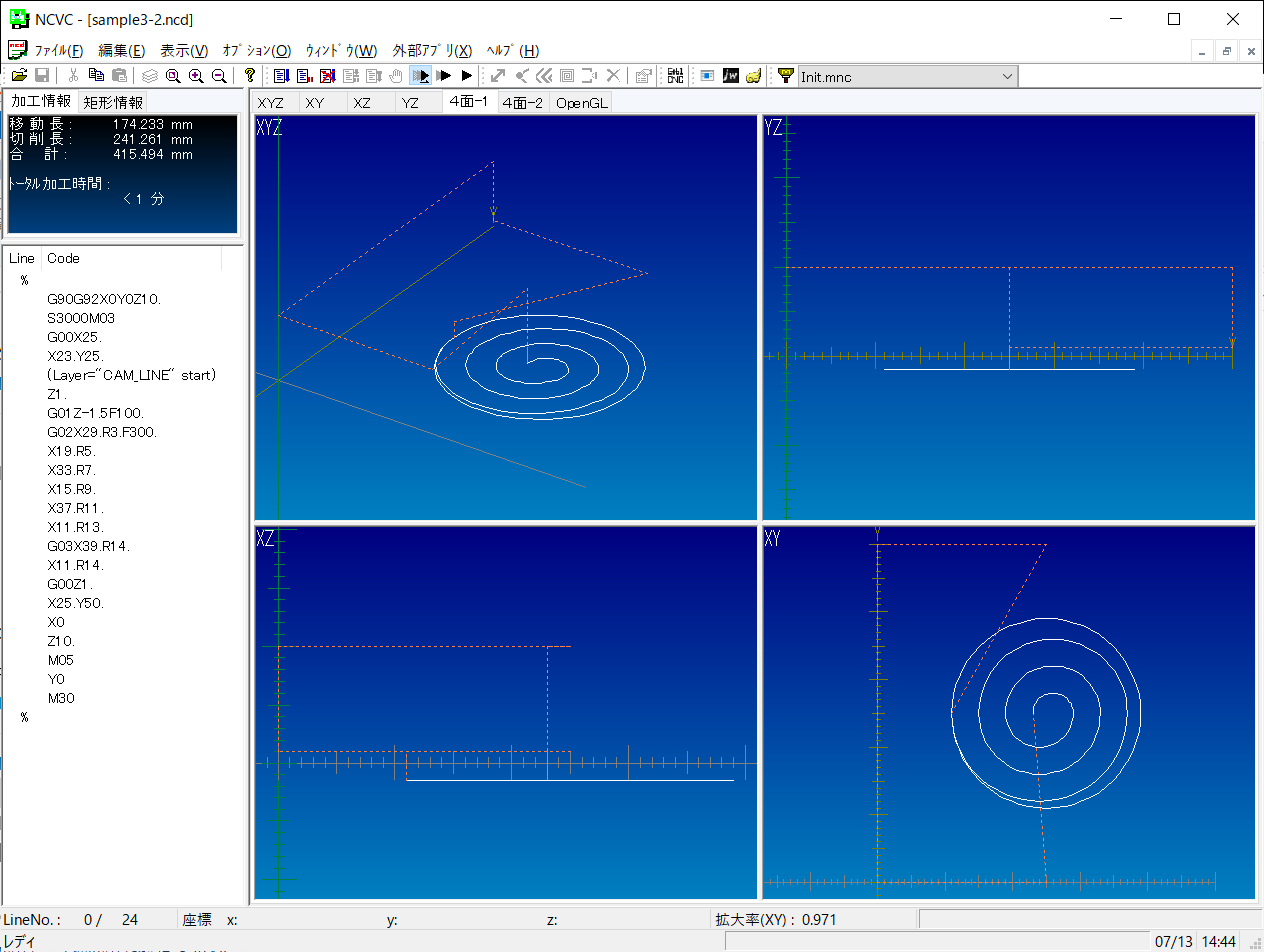
\includegraphics[scale=0.55]{No3/fig/sample3-2.png}
\caption{強制移動データを追加したGコードシミュレーション画面}
\label{fig:sample3-2.png}
\end{figure}

\begin{minipage}[t]{0.5\textwidth}
 図\ref{fig:sample3-2.png} のシミュレーション結果から,強制移動指示レイヤがR点で移動していることが解ります.
この設定は加工条件の[レイヤ]タブにあります.
今回の例では[イニシャル点復帰]が正解ですが,強制移動指示レイヤは大抵の場合,次の切削領域への移動制御に使われるため,
通常は[R点復帰]で問題無いと思います.
\end{minipage}
\begin{minipage}[t]{0.5\textwidth}
\vspace*{-2zh}
\begin{figure}[H]
\centering
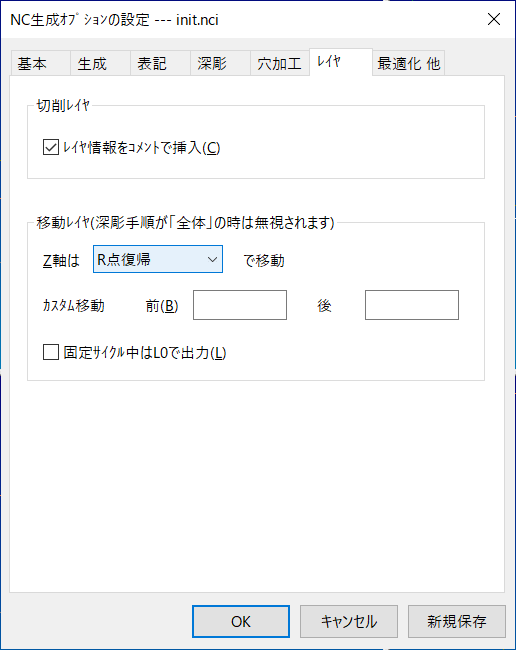
\includegraphics[scale=0.7]{No3/fig/move-setup.png}
\caption{強制移動指示レイヤのZ値設定}
\label{fig:move-setup.png}
\end{figure}
\end{minipage}

\begin{itembox}[l]{ここまでの【まとめ】}
(1) 加工開始位置指示レイヤ
\begin{itemize}
\item 加工開始位置を円で示す,またはアプローチ線を作図
\item 円や線は切削データと繋がって無くても良い
\end{itemize}
(2) 強制移動指示レイヤ
\begin{itemize}
\item 切削データが途切れ,次の切削領域へ移動するとき,参照される
\item 切削データと繋がっていなければならない
\item 強制移動指示レイヤのZ値は加工条件の設定による
\end{itemize}
\end{itembox}

\subsection{Gコード(文字)の埋め込み}
\label{sec:moji}
 NCVCで生成されるGコードは,基本的に位置決めと直線・円弧補間のG00~G03,固定サイクルG81~の一部だけです.
ここでは工作機械の特殊コード(例えばATCによるツール交換コード)やカスタムマクロ呼び出しコードなど,
生成されるGコードに任意の文字列を埋め込む方法を解説します.

\begin{minipage}[t]{0.5\textwidth}
 作図方法は至極簡単.図\ref{fig:moji.pdf} に示すように,埋め込みたいオブジェクト(線や円弧)の端点に文字を作図するだけです.
文字データは原点レイヤ以外,すなわち,切削レイヤと2つの移動レイヤ,
それから【\ref{sec:move} 移動レイヤ】の節で解説した最後のレイヤである[コメント文字列挿入用レイヤ](p.\pageref{fig:ReadSetup3.png} 図\ref{fig:ReadSetup3.png})に作図することができます.

 埋め込みタイミングは,文字専用レイヤである[コメント文字列挿入用レイヤ]が先に参照され,次に各レイヤタイプに属する文字データが参照されます.
[コメント文字列挿入用レイヤ]に書かれた文字はその名の通りGコードに対するコメントと見なされ,カッコで括られます.その他のレイヤに書かれた文字はそのまま出力されます.
なお,文字データは1行で作図する必要がありますが,複数行の任意Gコードを埋め込みたい場合は改行位置で ``\,\textbackslash n\,'' と入力して下さい.
\end{minipage}
\begin{minipage}[t]{0.5\textwidth}
\vspace*{-1zh}
\begin{figure}[H]
\centering
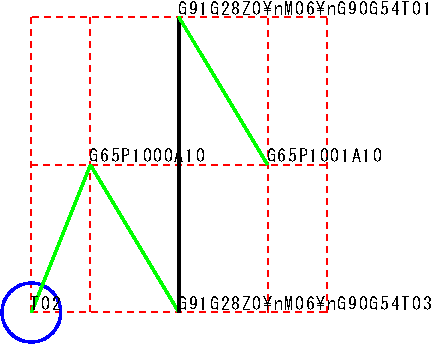
\includegraphics{No3/fig/moji-crop.pdf}
\caption{文字埋め込みサンプル}
\label{fig:moji.pdf}
\end{figure}
\end{minipage}

 図\ref{fig:moji.pdf} の作図から生成されるGコードは以下の通りです.
反転部分が文字情報から拾われたデータです.
作図は簡単ですが,文字を埋め込むレイヤと場所(タイミング)には若干知恵を絞る必要があります.

\begin{minipage}[t]{0.5\textwidth}
\begin{screen}
{\small\texttt{\%\\[-0.5zh]
G90G54G92X0Y0Z10.\\[-0.5zh]
M8\\[-0.5zh]
M68\\[-0.5zh]
S3000M3\\[-0.5zh]
\colorbox{black}{\textcolor{white}{T02}}\\[-0.5zh]
G00X10.Y25.\\[-0.5zh]
\colorbox{black}{\textcolor{white}{G65P1000A10}}\\[-0.5zh]
X25.Y0\\[-0.5zh]
\colorbox{black}{\textcolor{white}{G91G28Z0}}\\[-0.5zh]
\colorbox{black}{\textcolor{white}{M06}}\\[-0.5zh]
\colorbox{black}{\textcolor{white}{G90G54T03}}\\[-0.5zh]
Z1.\\[-0.5zh]
G01Z-2.F100\\
 右へ続く$\nearrow$
}}
\end{screen}
\end{minipage}
\begin{minipage}[t]{0.5\textwidth}
\begin{screen}
{\small\texttt{Y50.F300\\[-0.5zh]
\colorbox{black}{\textcolor{white}{G91G28Z0}}\\[-0.5zh]
\colorbox{black}{\textcolor{white}{M06}}\\[-0.5zh]
\colorbox{black}{\textcolor{white}{G90G54T01}}\\[-0.5zh]
G00Z1.\\[-0.5zh]
X40.Y25.\\[-0.5zh]
\colorbox{black}{\textcolor{white}{G65P1001A10}}\\[-0.5zh]
Z10.\\[-0.5zh]
M9\\[-0.5zh]
M5\\[-0.5zh]
X0Y0\\[-0.5zh]
M30\\[-0.5zh]
\%
}}
\end{screen}
\end{minipage}

\begin{figure}[H]
\centering
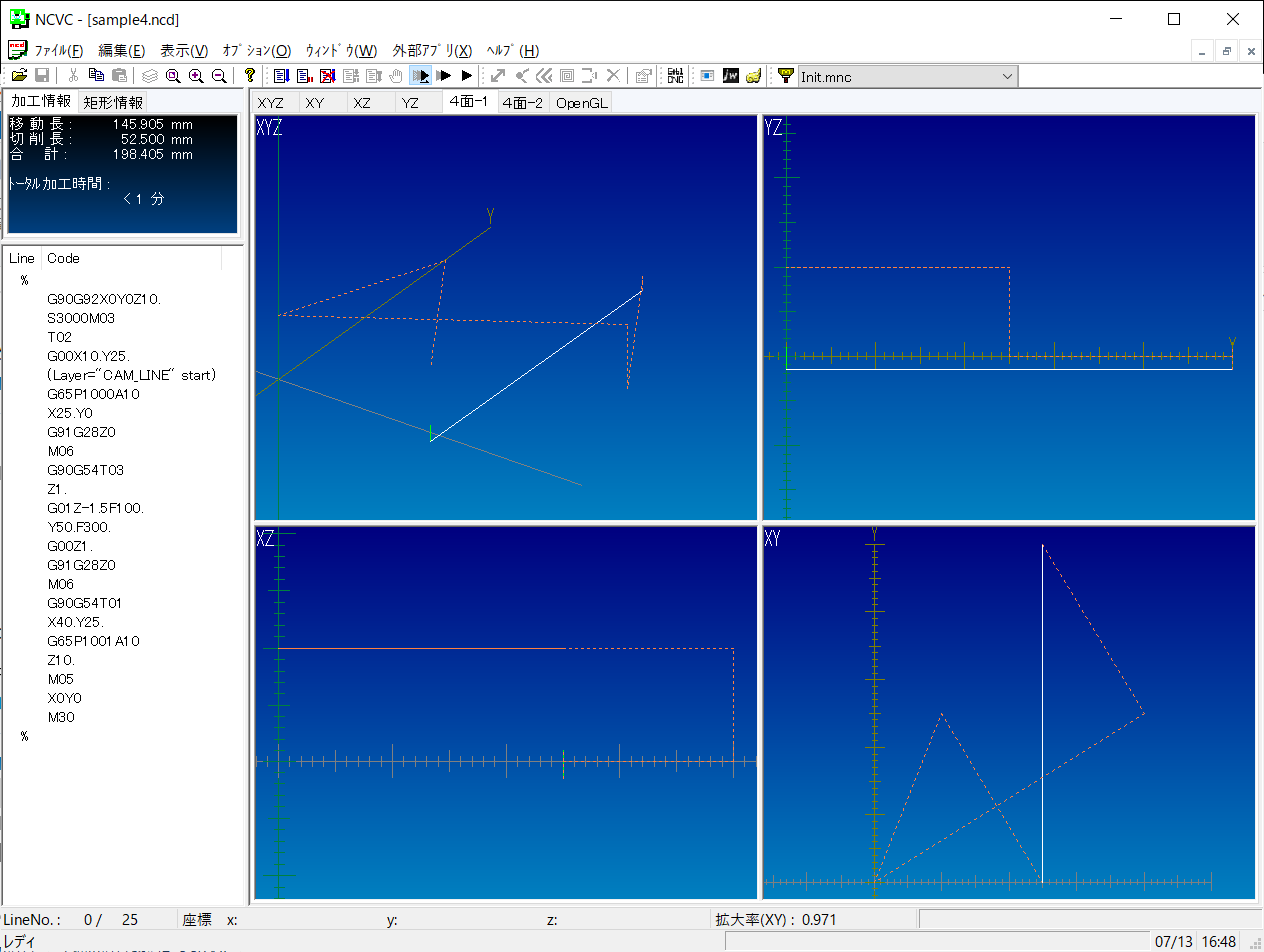
\includegraphics[scale=0.55]{No3/fig/sample4.png}
\caption{Gコードシミュレーション画面}
\label{fig:sample4.png}
\end{figure}

\subsection{深彫切削(Z軸ステップ切削)}
\label{sec:deep}
 ここでは[深彫切削]を解説します.
細い刃物での切削で1回の切り込み量に制限がある場合等,Z軸を段階的に下げて切削するコードを生成することができます.

\begin{minipage}[t]{0.5\textwidth}
 深彫切削は加工条件で指示します.
サンプルデータは【\ref{sec:DesignCAD} CADでの作図】を使いましょう.
同じく【\ref{sec:init.nci} 加工条件の設定】の要領で条件ファイルを開き,
[深彫]のタブをクリックして下さい(図\ref{fig:deep.png}).

 ポイントは2点.
まず[基本切り込み]の値ですが,ここでは ``\,1回目の切り込み量\,'' と解釈して下さい.
これは基本タブから参照されている値です.
このタブで値の変更はできません.

 次に深彫切削グループ一連の設定.
[最終切り込み]で最終的に必要な深さ,[切り込みステップ]にて刃物が一度に切り込む量を指定します.
とりあえずこの設定情報でGコードを生成してみると,図\ref{fig:deep.png} のようになります.

 その他の加工条件で代表的なもの.
[手順]は連続線グループを先に彫り進める(一筆)か,同一Z値で全体を彫り進める(全体)かの設定.
[方向]は次のZ値を切削するときにそのまま戻る(往復)か,一旦最初の加工座標まで戻る(一方)かの設定です.
いずれもシミュレーション画面で明確に出ますので,状況に応じて設定して下さい.
残りの設定は【リファレンス】で解説します.
\end{minipage}
\begin{minipage}[t]{0.5\textwidth}
\vspace*{-2zh}
\begin{figure}[H]
\centering
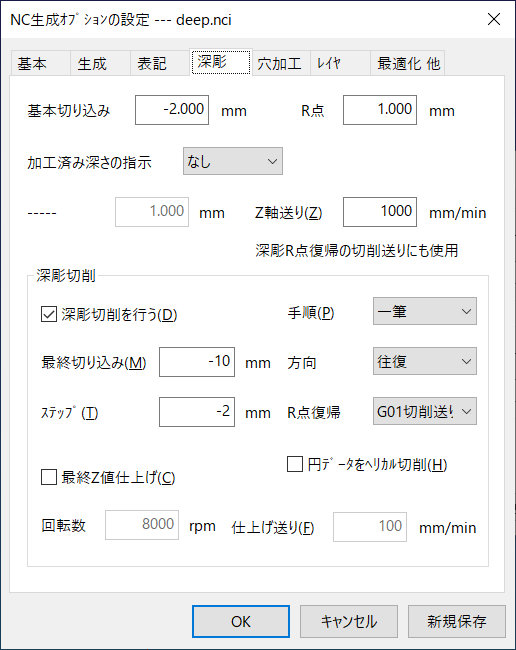
\includegraphics[scale=0.7]{No3/fig/deep-setup.png}
\caption{深彫の設定}
\label{fig:deep-setup.png}
\end{figure}
\end{minipage}

\begin{figure}[H]
\centering
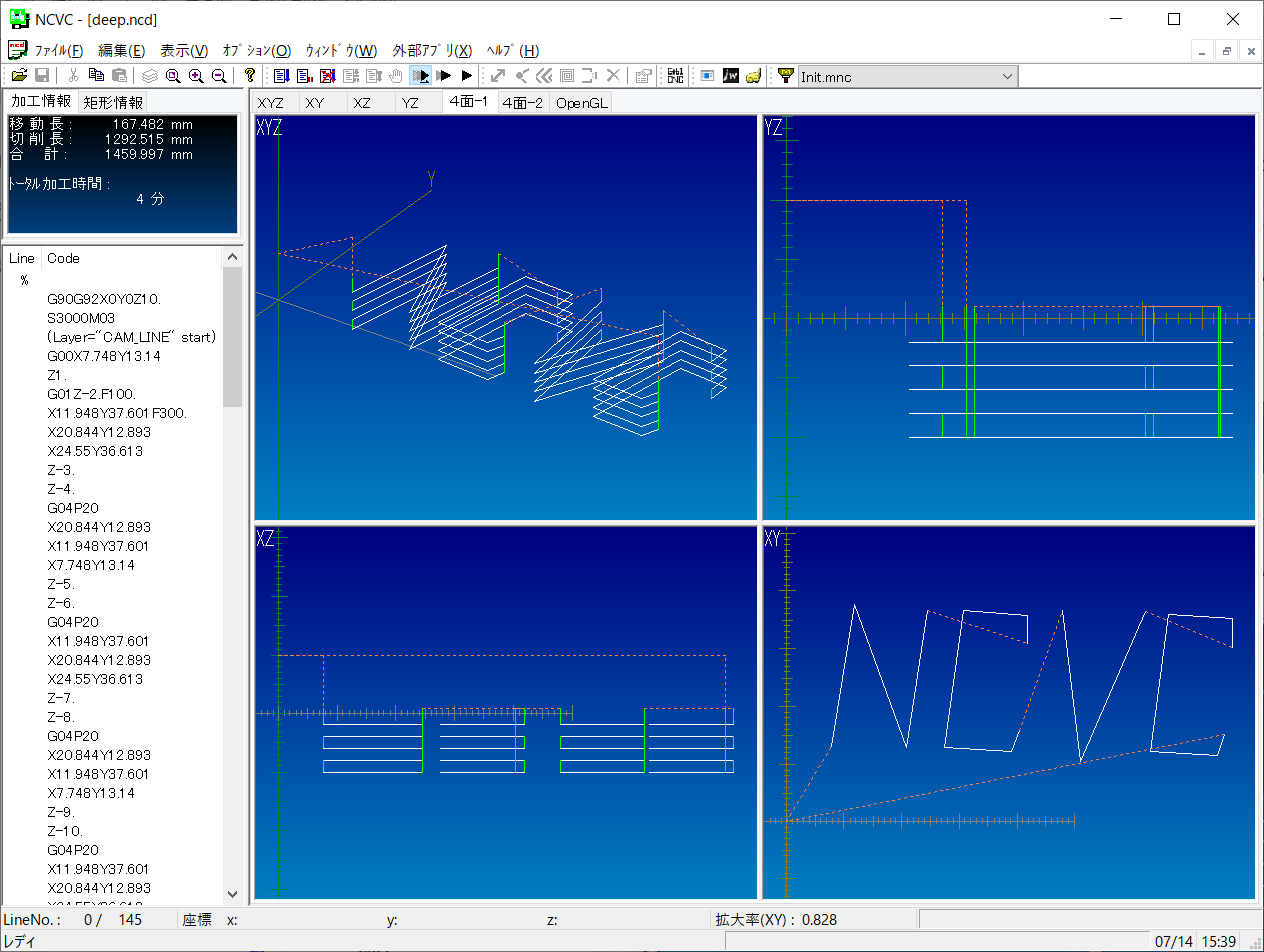
\includegraphics[scale=0.55]{No3/fig/deep.png}
\caption{深彫のシミュレーション結果}
\label{fig:deep.png}
\end{figure}

\newpage
\subsection{複数レイヤ処理(2.5D切削)}
\label{sec:multi-layer}
 これまで2次元CADで作図したデータと加工条件に示すZ値から2次元の加工データを生成してきました.
1つの切削レイヤに1つのZ値(加工条件)を対応させていたわけです.
ここでは,複数の切削レイヤを処理しそれぞれにZ値を割り当てることで,簡易2.5Dの切削データを生成する方法を解説します.

\subsubsection{レイヤごとのZ座標指定}
\label{sec:layer-z}

\begin{minipage}[t]{0.5\textwidth}
 図\ref{fig:25d.pdf} は一見して解りづらい図面ですが,上がXY平面図,下が側面図と考えて下さい.
側面図の半円が切削したい曲線ですが,これをXY平面におこすため,一定間隔(この例では1mm)で補助線を引き,さらに半円との交点でXY平面用に縦の補助線を引いています.
XY平面図では側面図からの補助線と工具径を考慮しながら切削パスを作図しています.
ただし,それぞれの切削パスがどのZ座標かを示すため,図\ref{fig:25d-layer.png} のように複数\footnotemark[1]
の切削レイヤに作図しています.
高さ30mmを1mm間隔で分割.徐々に外側へ広がっている様子が解ると思います.

 作図が終われば,各レイヤに名前を割り当てましょう.
特に切削レイヤには,それぞれが識別できるよう連番を振ります.
\end{minipage}
\begin{minipage}[t]{0.5\textwidth}
\vspace*{-2zh}
\begin{figure}[H]
\centering
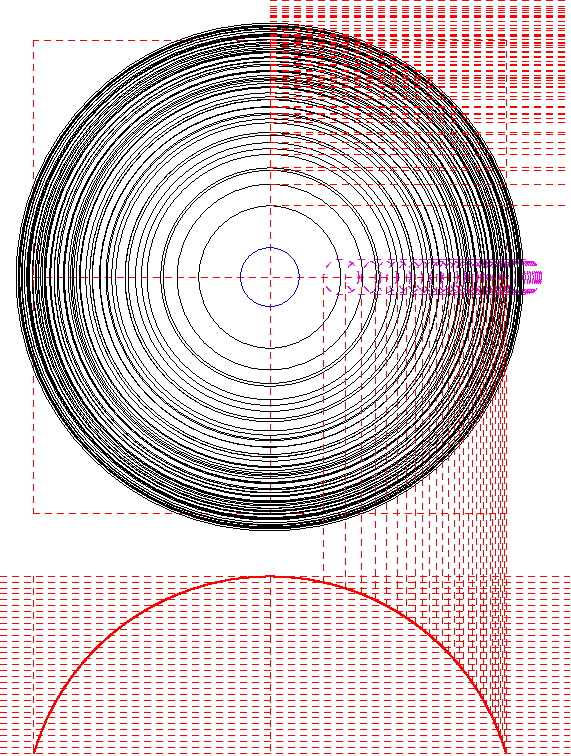
\includegraphics[width=\textwidth]{No3/fig/25d-crop.pdf}
\caption{複数レイヤのサンプル図形}
\label{fig:25d.pdf}
\end{figure}
\end{minipage}
\footnotetext[1]{Jw\_cadは1レイヤグループ16個のレイヤが割り当てられているので2つのレイヤグループを使用.30個の切削レイヤと原点・補助線レイヤで計32個のレイヤを使用しています.}

\begin{figure}[H]
\centering
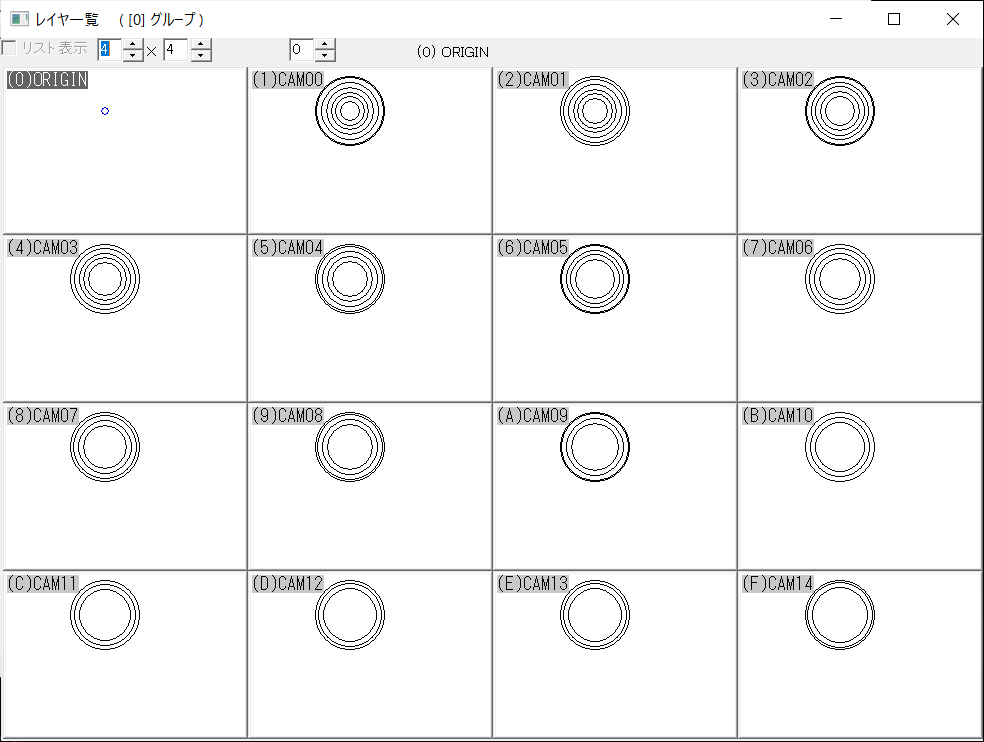
\includegraphics[scale=0.7]{No3/fig/25d-1.png}\\[2zh]
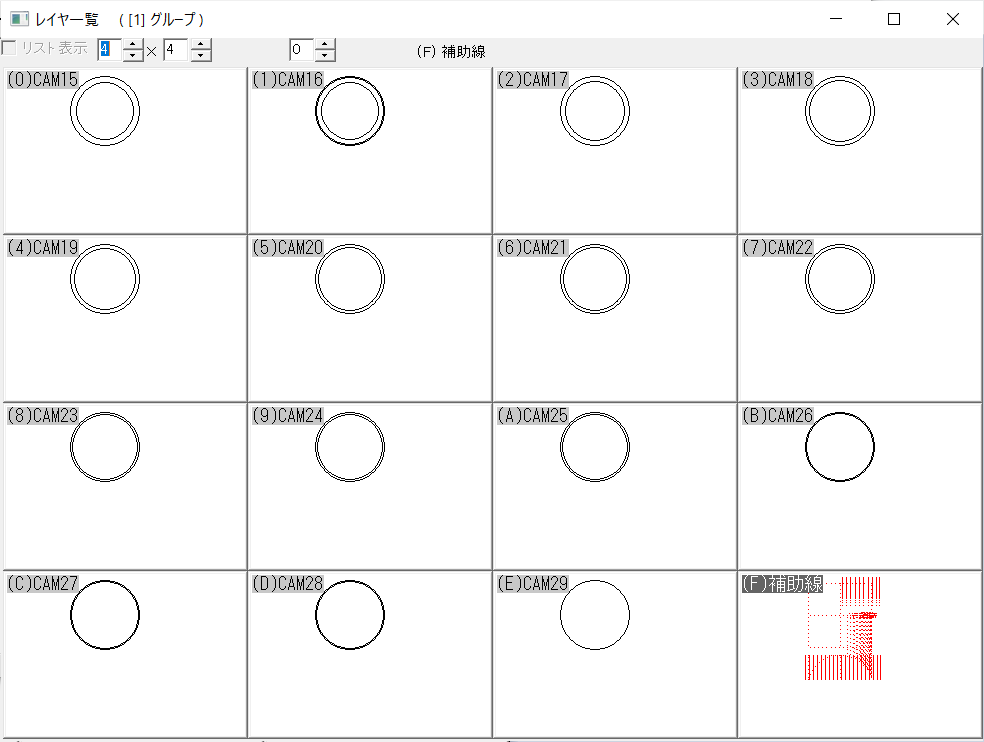
\includegraphics[scale=0.7]{No3/fig/25d-2.png}
\caption{複数レイヤのレイヤ一覧}
\label{fig:25d-layer.png}
\end{figure}

\begin{minipage}[t]{0.5\textwidth}
 次にこの作図データをNCVCに読み込ませるわけですが,図\ref{fig:ReadSetup.png} 読み込みレイヤ設定では単一の切削レイヤしか処理できません.
複数の切削レイヤを処理するには,図\ref{fig:25d-setup.png} のように正規表現\footnotemark[2]で認識文字列パターンを入力するか,
従来互換を選択し,「レイヤ名``\,CAM\,''を``\,部分一致\,''で``\,認識\,''する」と指定して下さい.
図\ref{fig:25d-setup.png} の入力例は「文字列``\,CAM\,''に続く数値(0~9)を認識」と解釈されます.

 読み込みレイヤが設定できれば,NCVCでCADデータを開きます.
図\ref{fig:25d-read.png} は\menu{表示>レイヤ}をクリックし,複数レイヤが読み込まれていることを確認しています.
\end{minipage}
\begin{minipage}[t]{0.5\textwidth}
\vspace*{-2zh}
\begin{figure}[H]
\centering
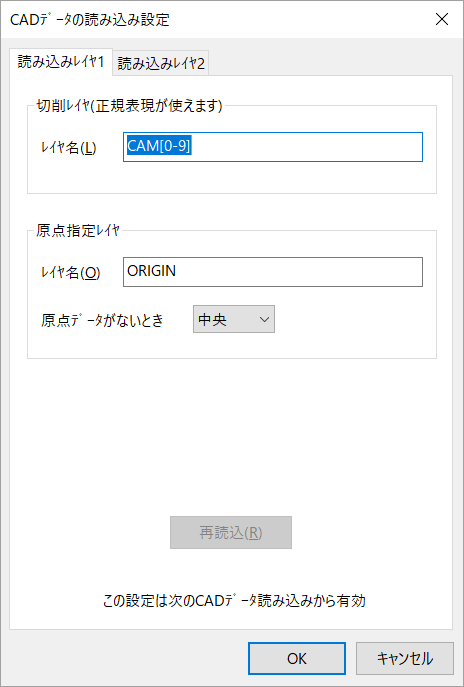
\includegraphics[scale=0.7]{No3/fig/25d-setup.png}
\caption{複数レイヤの読み込み設定}
\label{fig:25d-setup.png}
\end{figure}
\end{minipage}
\footnotetext[2]{[XXで始まる文字列]や[YYで終わる文字列]など,文字列のパターンマッチングを表現,コンピュータに指示するための表記のこと.
NCVCに限った話ではない.正規表現の解説はそれだけで1冊の本ができるほど様々な表記法があるので,覚える必要はない.}

\begin{figure}[H]
\centering
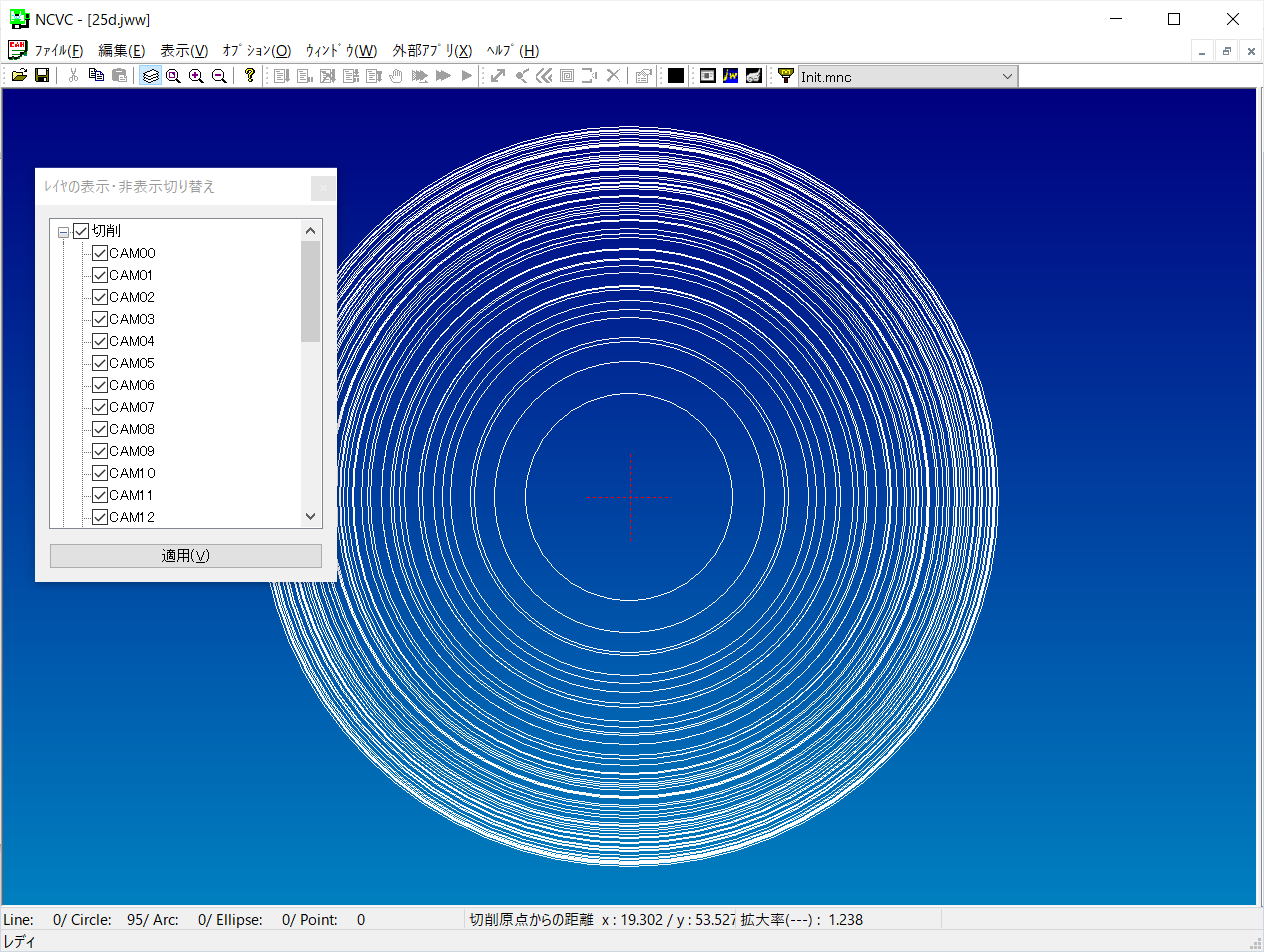
\includegraphics[scale=0.55]{No3/fig/25d-read.png}
\caption{複数レイヤの読み込み}
\label{fig:25d-read.png}
\end{figure}

 複数の切削レイヤにZ値を割り当てるには,\menu{ファイル>NCデータへの変換>レイヤごとのZ座標指定}
\footnote{複数の切削レイヤが読み込まれていないとこのメニューは選択できません}
をクリックし,図\ref{fig:25d-make1.png} のダイアログから行います.
NCデータの出力ファイル名と条件ファイルの指定は \ref{sec:basic}章と同じ.
[レイヤ名とZ座標との関係]は次に説明する設定を保存するファイル(nclファイル)です.
ここの編集ボタンをクリックすると図\ref{fig:25d-make2.png} のダイアログが表示されます.

 レイヤ名には読み込んだ切削レイヤの一覧が列挙されます.
[切り込みの自動設定]に[これ以降 ``\,-1\,''mmごとに]と入力し設定ボタンを押すと,CAM00~CAM29まで順に-1mmづつZ座標を設定できます.
この値は加工条件の切り込み
\footnote{【\ref{sec:init.nci} 加工条件の設定】を参照}
に置き換えられます.

 OKを押すと図\ref{fig:25d-make1.png} に戻ります.
図\ref{fig:25d-make2.png} で設定したZ値を保存しておきたい場合は,[レイヤ名とZ座標との関係]のファイル覧に適当な名前(フルパス名)を入力します.

\begin{minipage}{0.5\textwidth}
\begin{figure}[H]
\centering
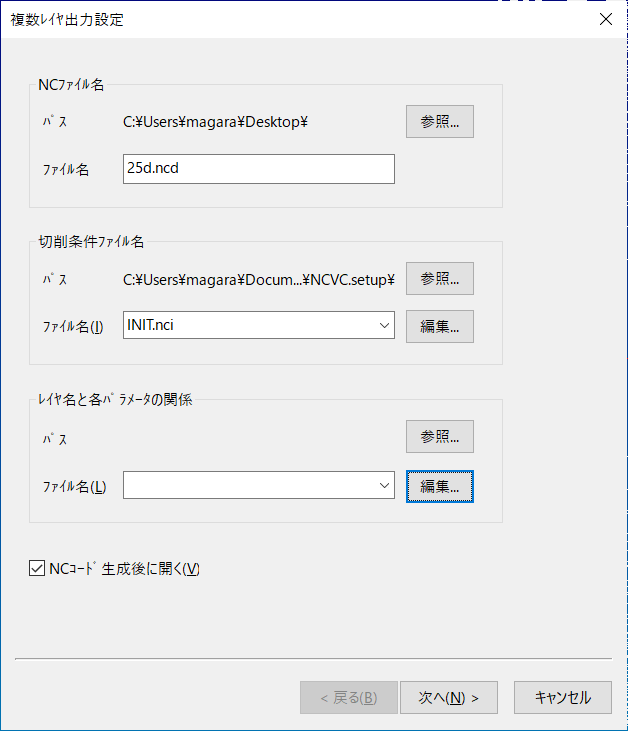
\includegraphics[scale=0.6]{No3/fig/25d-make1.png}
\caption{複数レイヤの設定}
\label{fig:25d-make1.png}
\end{figure}
\end{minipage}
\begin{minipage}{0.5\textwidth}
\begin{figure}[H]
\centering
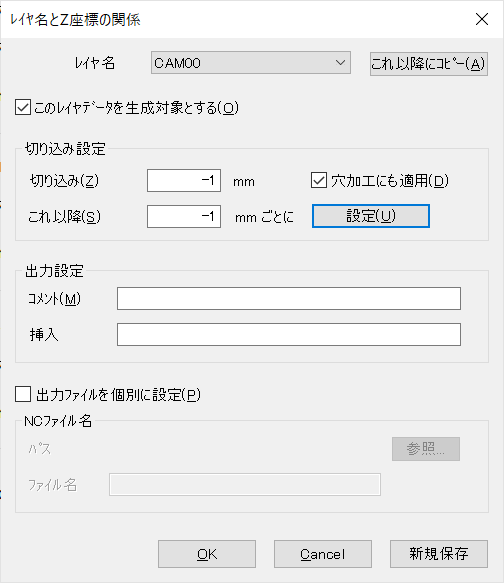
\includegraphics[scale=0.7]{No3/fig/25d-make2.png}
\caption{複数レイヤのZ値設定}
\label{fig:25d-make2.png}
\end{figure}
\end{minipage}

\vspace*{2zh}
 全ての設定が完了し図\ref{fig:25d-make1.png} でOKボタンを押すと,図\ref{fig:25d.png} の通り簡易2.5Dの切削データが生成できました.

\begin{figure}[H]
\centering
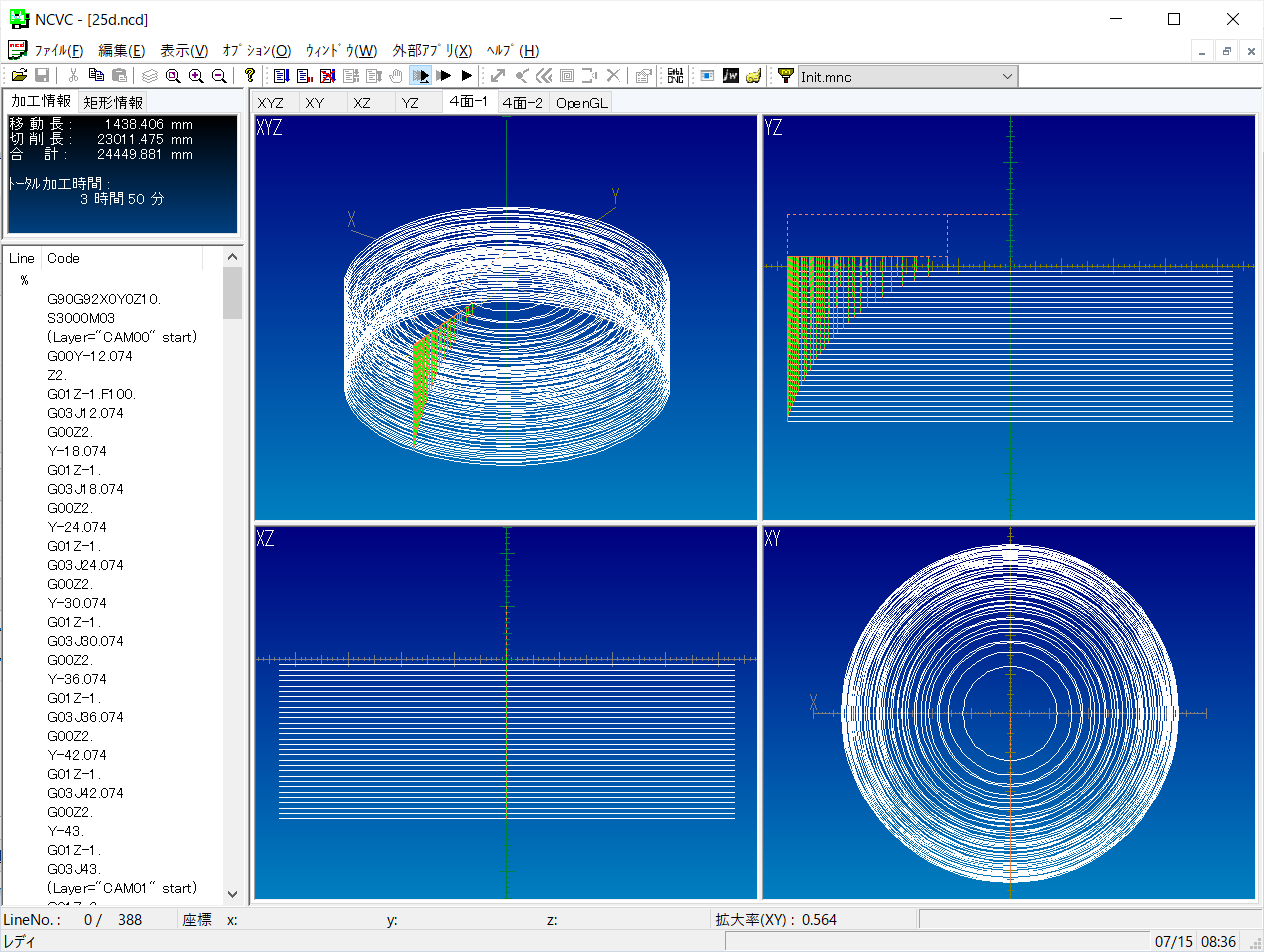
\includegraphics[scale=0.55]{No3/fig/25d.png}
\caption{複数レイヤによる簡易2.5Dシミュレーション画面}
\label{fig:25d.png}
\end{figure}

\subsubsection{レイヤごとの切削条件}

\begin{minipage}[t]{0.49\textwidth}
 【\ref{sec:layer-z} レイヤごとのZ座標指定】では,その名の通り複数の切削レイヤにZ値だけを強制的に設定しました.
加工条件は1つだけなので,主軸回転数や送り速度等は全て同じです.
これらをもレイヤごとに設定したい,例えば図\ref{fig:shima-img.png} のような島加工で外側と内側の切削条件を変えたい場合,
[レイヤごとの複数条件]を使います.
\end{minipage}
\begin{minipage}[t]{0.02\textwidth}
 
\end{minipage}
\begin{minipage}[t]{0.49\textwidth}
\vspace*{-2zh}
\begin{figure}[H]
\centering
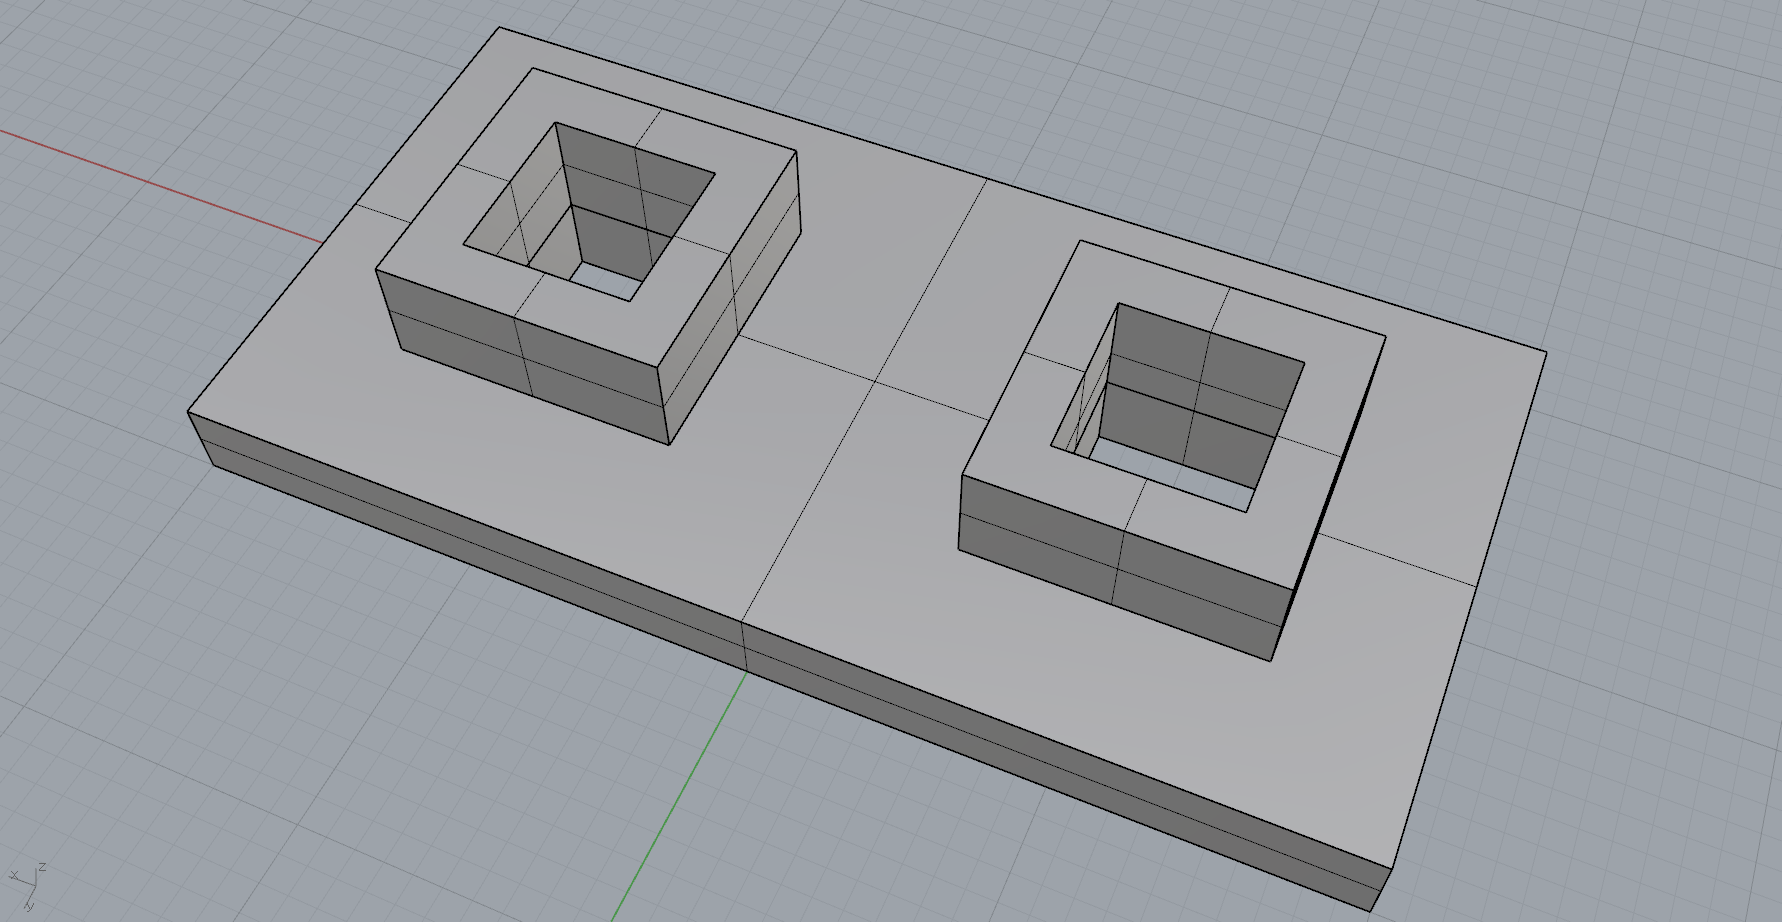
\includegraphics[width=\textwidth]{No3/fig/shima-img.png}
\caption{島加工切削例}
\label{fig:shima-img.png}
\end{figure}
\end{minipage}

\vspace*{2zh}
 \menu{ファイル>NCデータへの変換>レイヤごとの複数条件}をクリックすると
図\ref{fig:25d-make3.png} のダイアログが表示されます.基本的には図\ref{fig:25d-make1.png} と同じですが,
加工条件をレイヤごとに設定するため,切削条件ファイルは明細の方に移動しています.
前節同様[レイヤ名とZ座標との関係]の編集ボタンを押すと図\ref{fig:25d-make5.png} のダイアログが表示されるので,
各レイヤごとに条件ファイルを割り当てます.

 各レイヤごとにZ値を指定するか加工条件を指定するかだけの差で前節と同じです.
シミュレーション画面も割愛します.

\begin{figure}[H]
\begin{minipage}[t]{0.5\textwidth}
\centering
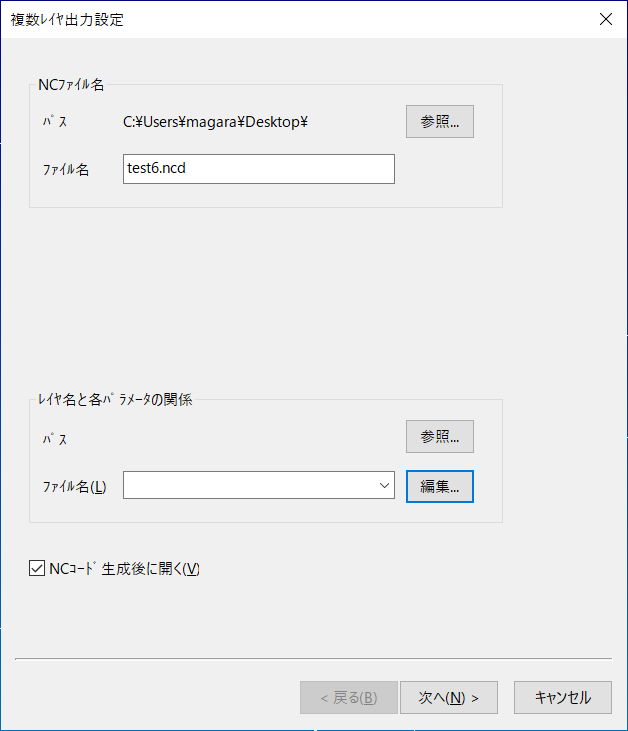
\includegraphics[scale=0.6]{No3/fig/25d-make3.png}
\end{minipage}
\begin{minipage}[t]{0.5\textwidth}
\centering
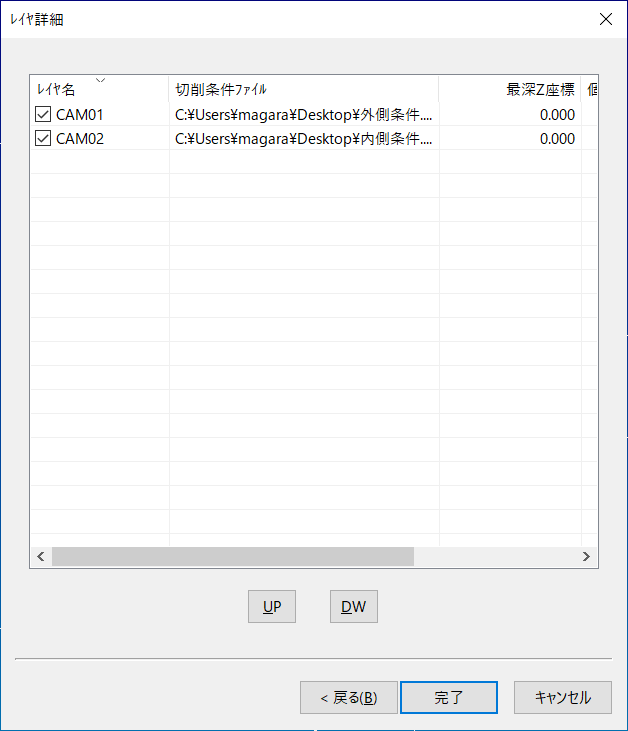
\includegraphics[scale=0.6]{No3/fig/25d-make4.png}
\end{minipage}
\caption{複数レイヤのZ値設定}
\label{fig:25d-make3.png}
\end{figure}

\begin{figure}[H]
\centering
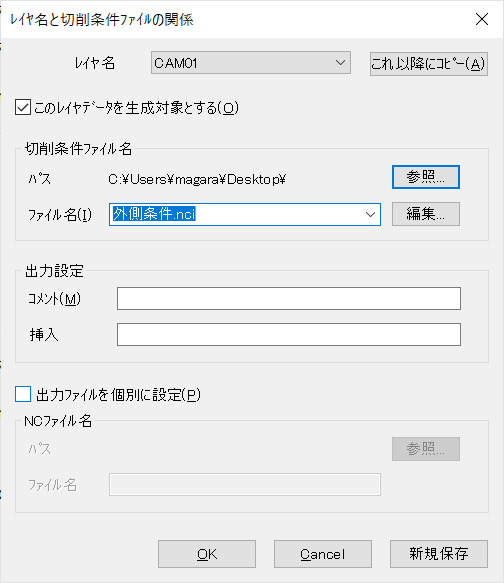
\includegraphics[scale=0.7]{No3/fig/25d-make5.png}
\caption{複数レイヤの加工条件割り当て}
\label{fig:25d-make5.png}
\end{figure}

\subsubsection{個別出力について}
 図\ref{fig:25d-make2.png} および図\ref{fig:25d-make5.png} の
[出力ファイルを個別に設定]にチェックを入れると,各レイヤごとに出力するファイルを指示できます.

\newpage
\begin{itembox}[l]{ここまでの【まとめ】}
\begin{itemize}
\item 複数レイヤによる簡易2.5D切削であってもXZまたはYZ平面での指示はできない
\end{itemize}
\end{itembox}
